\section{Calibration Target Design}
A contiguous calibration target was chosen initially for beam direction estimation. However, the variable albedo due to ink created structured noise. This caused estimates of beams partially overlapping black regions to become biased towards the white regions. As a result, a window was added to the target allowing all centroiding estimates to occur on a surface of constant albedo. See Figure \ref{fig:target_window}.

\begin{figure}
    \centering
    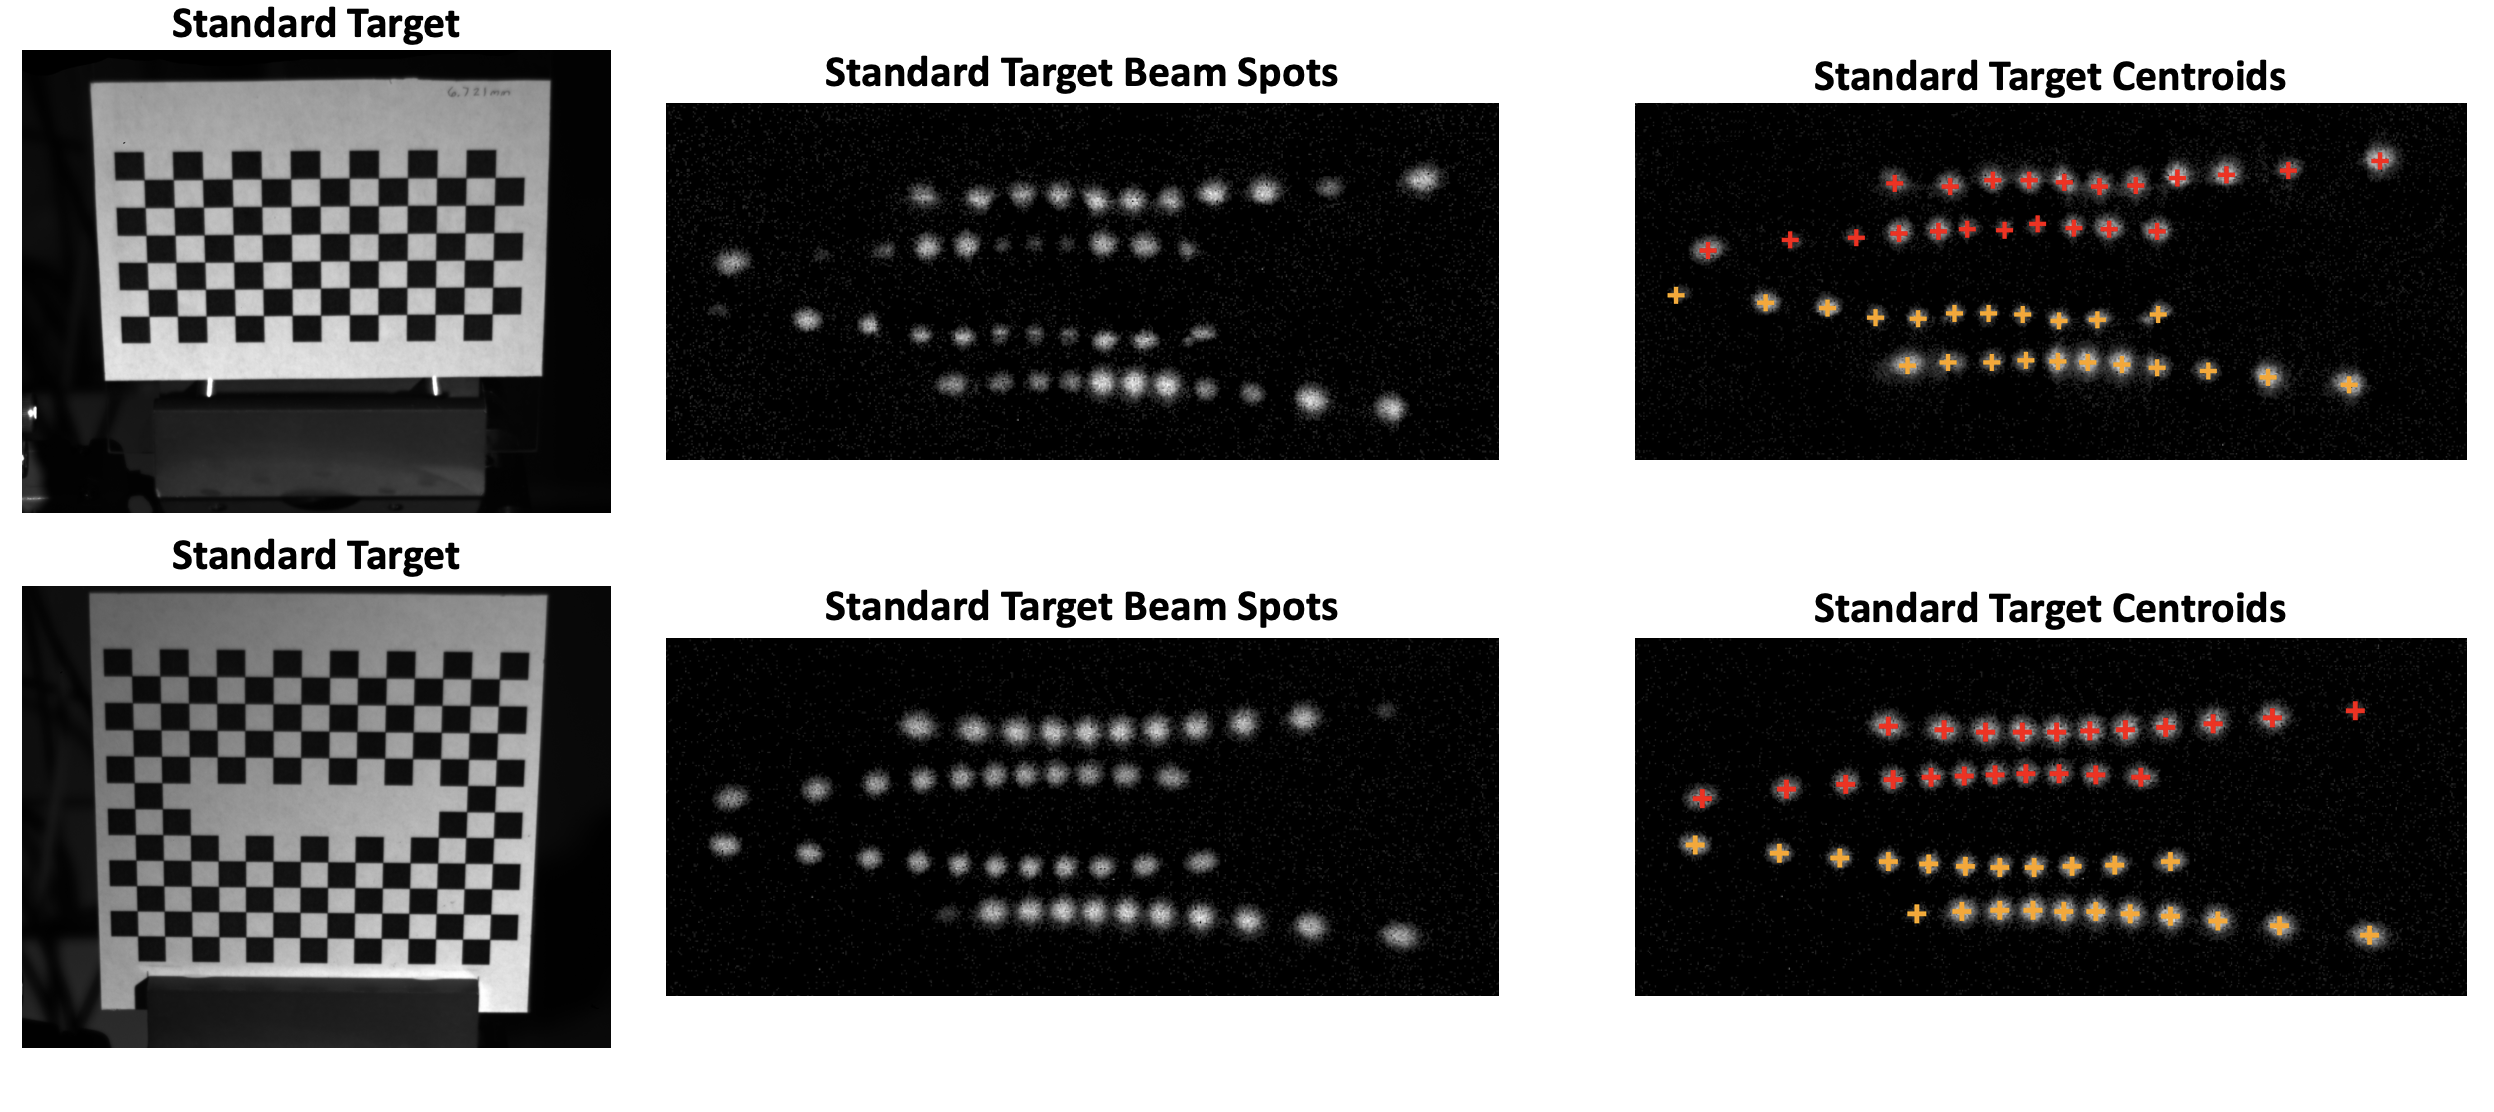
\includegraphics[width=\linewidth]{figures/CalTarget_Std_vs_Windowed.png}
    \caption{Top row: Original target used for calibration caused irregular beam spot shapes which produced noisy centroids. Bottom row: Windowed target used now to avoid albedo issues when imaging beam spots.}
    \label{fig:target_window}
\end{figure}